\documentclass[
	headsepline=on,
	footsepline=on,
	twoside=off,
	abstract=on,
	DIV=10
]{scrreprt}

\usepackage[utf8]{inputenc}
\usepackage{graphicx}
\usepackage[english, french]{babel}
\usepackage{multirow}
\usepackage[dvipsnames]{xcolor}
\usepackage[hidelinks]{hyperref}
\usepackage{mdframed}
\usepackage{pgfplotstable}
\usepackage{tikz-3dplot}
\usepackage[OT1]{fontenc}
\usepackage{lipsum}
\usepackage{float}
\usepackage{pdfpages}
\usepackage{amsmath}


\definecolor{link}{HTML}{4169E1}

\usepackage[bottom=2cm,footskip=8mm]{geometry}

\newmdenv[
rightline=false,
topline=false,
bottomline=false,
backgroundcolor=BurntOrange!5,
fontcolor=BrickRed,
linecolor=Red,
linewidth=1pt]{problem}


\newmdenv[
rightline=false,
topline=false,
bottomline=false,
backgroundcolor=ForestGreen!5,
fontcolor=OliveGreen,
linecolor=Green,
linewidth=1pt]{result}


\newmdenv[
rightline=false,
topline=false,
bottomline=false,
backgroundcolor=Cyan!5,
fontcolor=Blue,
linecolor=NavyBlue,
linewidth=1pt]{info}

%Gestion des images

\newcommand{\img}[1]{
\begin{figure}[H]
	\centering
	\includegraphics[width=0.8\textwidth]{#1}	
\end{figure}
}

% Gestion d'abstracts multiples

\newenvironment{abstractpage}
{\cleardoublepage\vspace*{\fill}\thispagestyle{empty}}
{\vfill\cleardoublepage}

\renewenvironment{abstract}[1]
{\bigskip\selectlanguage{#1}%
	\begin{center}\bfseries\abstractname\end{center}}
{\par\bigskip}

% Gestion des keywords

\newcommand{\keywords}{\sffamily\textit{Keywords : }\bfseries}

%Page style

\pagestyle{headings}
\pagenumbering{arabic}


%Title page

\titlehead{
	
\includegraphics[width=0.25\textwidth]{pics/logo_UNICAEN.png}
}
\subject{
	\small
	Université de Caen Normandie\\
	UFR des Sciences\\
	Département Informatique\\
	\hfill\\
	3ème année de licence d'informatique
}
\title{
	%\hrulefill
	\vfill\\
	\Huge \bfseries PolTron: La coalition
}
\subtitle{
	Expérimentations sur coalition d'IA via le jeu Tron\\
	\hfill
}
\author{
	\small
	
\includegraphics[ height=0.12\textheight]{pics/logo_long_promo.png}\\
	\hfill\\
	Christopher JACQUIOT, Vincent DE MENEZES, \\ Alexis MORTELIER, Walid IDOUCHE
}
\date{}
\publishers{
	\small
	\begin{minipage}{0.6\textwidth}
		Tuteur du projet: Gregory BONNET\\
		\\
		Jury : --\\
		\textit{(si composition du jury connue)}
	\end{minipage}
	\hfill
	\begin{minipage}{0.35\textwidth}
		Année universitaire : 2018 / 2019\\
		\\
		Soutenu le -- mars 2019\\
		\textit{(si date connue)}
	\end{minipage}
}

\makeglossary

\begin{document}
	\maketitle
	
	
	\pagenumbering{roman}
	
	
	\tableofcontents
	\listoffigures

	\chapter*{Remerciements}
		\paragraph{} 
			Nous tenons à remercier notre tuteur M. Gregory BONNET, pour la proposition de ce sujet passionnant.
					
	\clearpage
	
	\begin{abstractpage}
		\begin{abstract}{french}
			Dans ce projet mêlant intelligence artificielle, simulation et analyse, nous allons devoir créer un jeu inspiré de Tron sur lequel nous allons faire jouer plusieurs équipes, une coalition et un joueur seul, leur donnant une différence d'intelligence telle que le joueur solo sera le plus intelligent, et nous allons ensuite devoir analyser les résultats de leurs parties pour déterminer les paramètres les plus optimaux pour que cette coalition gagne contre le joueur seul. Pour réaliser cela nous allons avoir recours à diverses technologies pour résoudre les divers problèmes auquels nous allons nous confronter. Parmi ces technologies, le python sera utile pour réaliser rapidement notre modèle et notre interface, le Sqlite avec sa portabilité et sa forte intégration avec la plupart des langages sera primordial pour stocker et manipuler les données résultantes de nos simulations, et le langage d'analyse statistique R sera un grand atout pour aider à raisonner rapidement à partir de ces résultats.

		\end{abstract}
	
		\begin{abstract}{english}
			In this project about artificial intelligence, simulation and analysis, we will have to make an Tron-inspired game on which we will make two teams fight each other, a coalition and an alone player, both having different intelligence levels, the solo player being the most intelligent, and then analyze the results of their games to determine the optimum parameters to make the coalition win against the solo player. To realize this we will need to make good use of diverse technologies to deal with the problems we will face. Amongst thos technologies, Python will be useful to produce efficiently both our model and interface, Sqlite thanks to it's portability and deep integration with most languages will be primordial to store and manipulate the data resulting from our simulations, and the statistical analysis programming language R will be a great asset to help reason quickly from those results.

		\end{abstract}
		\hfill\\
		\keywords{AI analysis simulation Tron }
	\end{abstractpage}

	
	\pagenumbering{arabic}
	
	\part{Analyse du projet}
		
	\chapter{Introduction}
		\section{Objectif général du projet}
		\paragraph{Quel est le problème à régler?}
		Dans un jeu de Tron dont les règles sont explicitées dans la partie sur le modèle, nous allons faire jouer deux équipes:
		
		\begin{itemize}
			\item Un joueur seul et intelligent
			\item Une coalition de joueurs moins intelligents
		\end{itemize}
		
		Le but est d'analyser les meilleurs paramètres pour que notre coalition soit statistiquement la plus efficace contre le joueur seul, si une tendance se dégage de nos simulations.
		
		En d'autres termes, nous allons tenter de répondre à la question:
		
		
		\begin{problem}
			\sffamily
			Combien faut-il d'idiots pour prendre l'avantage sur un joueur plus intelligent?
		\end{problem}
	
		\section{Objectifs à atteindre}
		\paragraph{Simulateur} 
		Une interface permettant de suivre la progression de la simulation est très importante pour estimer quand terminent nos simulations.
		
		\paragraph{Modèle de jeu}
		Le moteur de jeu devra être le plus optimisé possible pour éviter de couter en temps de simulation pour l'heuristique et permettre le calcul d'un maximum de parties.
		
		\paragraph{IA et son heuristique}
		L'intelligence artificielle va devoir être capable de se défendre et d'attaquer l'équipe adverse de façon efficace et l'heuristique devra être optimisée au possible.
		
		\paragraph{Stockage de masse}
		Au vu des grandes quantités de données potentielles, une base de donnée bien structurée avec des vues permettant de faciliter l accès aux informations pertinentes pour l'analyse sera primordiale.
		
		\paragraph{Analyse statistique}
		Nous allons devoir faciliter la visualisation et le travail sur nos données afin de permettre de se concentrer sur l'analyse plutôt que sur les outils d'analyse. Il sera donc important d'unifier au possible les moyens d'analyse des données et de rédaction d'analyses pour augmenter notre efficacité.
		
		
		\part{Cahier des charges}
		

		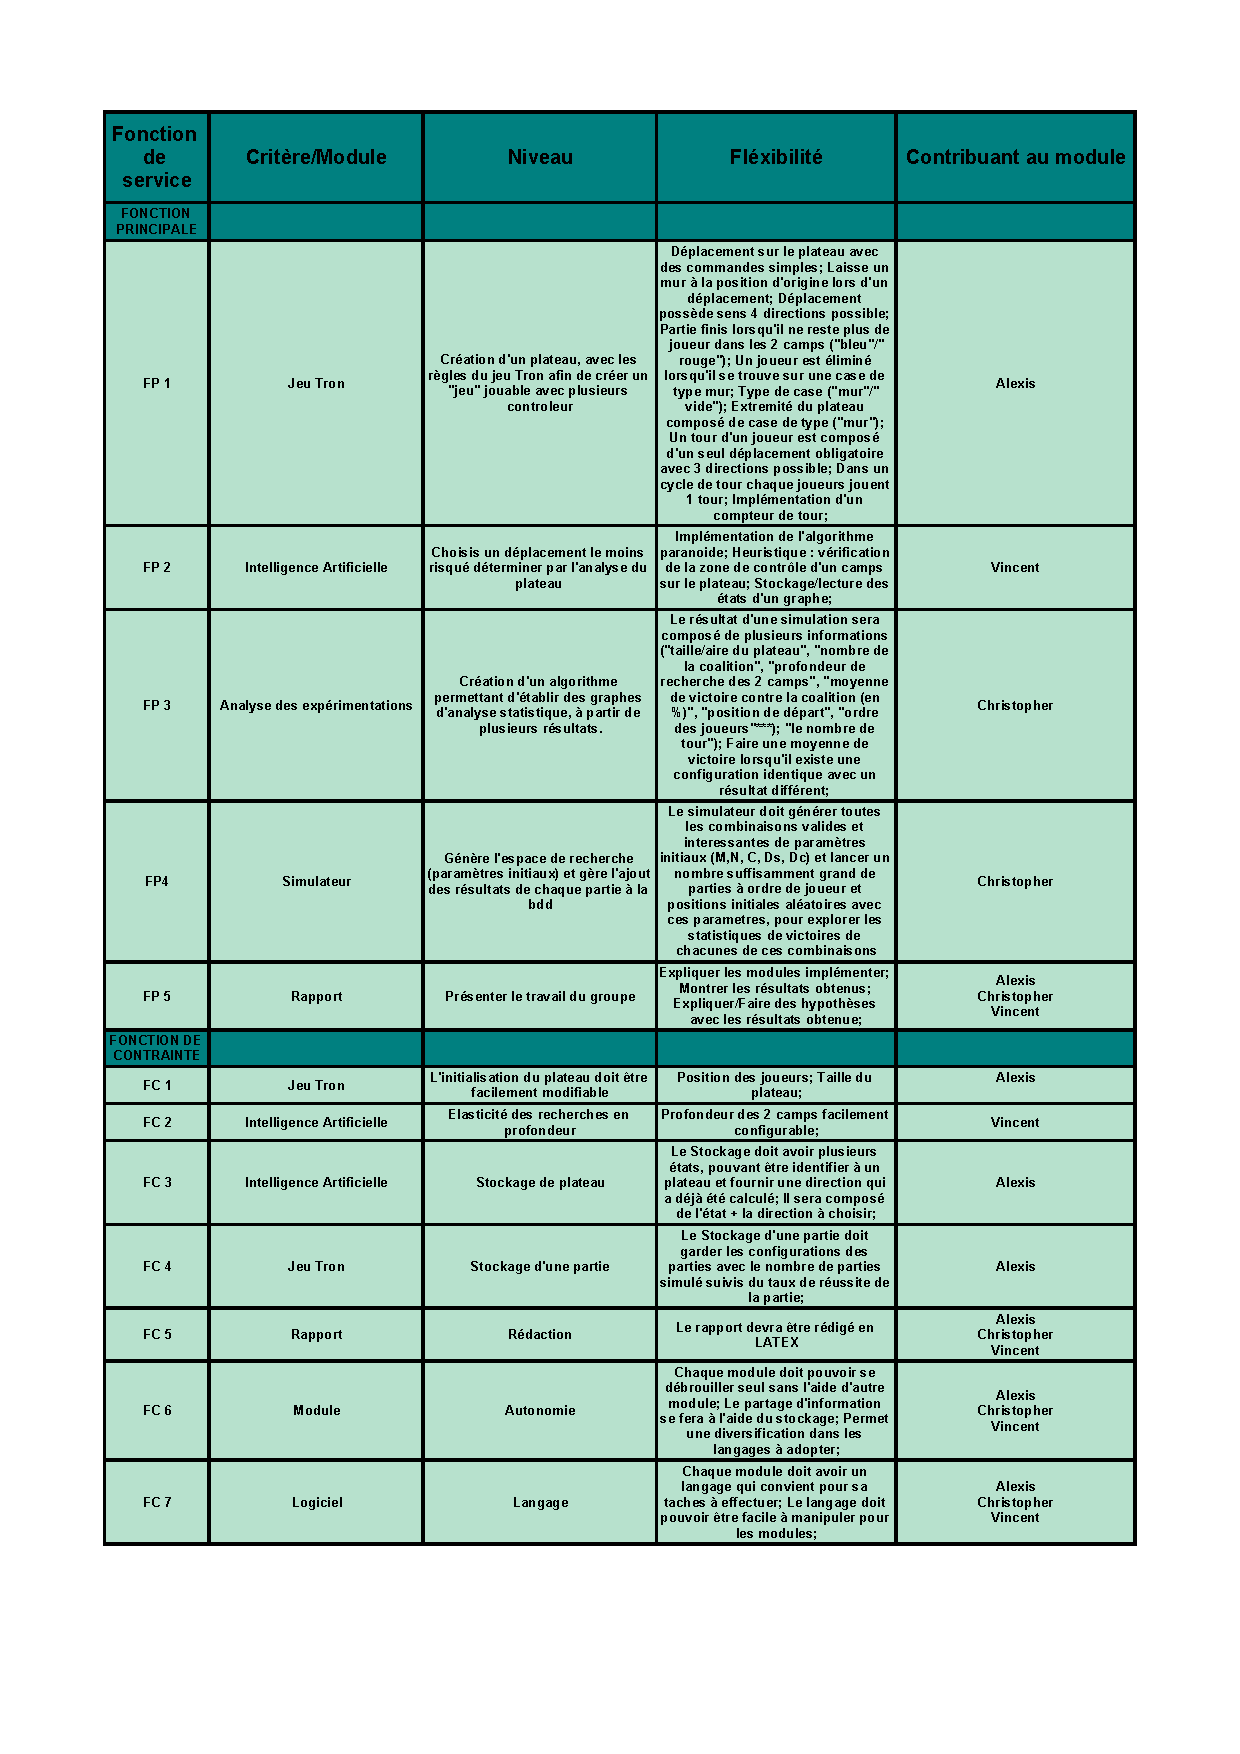
\includepdf[pages=-]{./data/cahier.pdf}
		
		\section{Spécifications}
			\subsection{Spécification des paramètres de simulation}
				
				\begin{figure}[H]
					\centering
					\begin{tabular}{l l}
						Paramètre de simulation&Signification\\\hline
						M & Longueur du terrain\\
						N & Largeur du terrain\\
						C & Nombre de joueurs dans la coalition\\
						Ds & Intelligence du joueur solo\\
						Dc & Intelligence des joueurs de la coalition
					\end{tabular}
					\caption{Nomenclature des paramètres de jeu}				
				\end{figure}
				
			\subsection{Contraintes techniques}
				\paragraph{Temps imparti réduit}
				
				Suite à une annulation de la matière puis à la réouverture de celle ci, le temps imparti pour ce projet as été considérablement amoindri.
				
				Nous avons environ 5 semaines pour mener ce projet à terme à compter du 31 janvier 2019.
				Il est donc nécessaire de réduire un maximum les temps de développement pour le mener à bien.
				
				Cela a mené à la nécessité d'évaluer nos options de façon la plus pragmatique possible en termes de coûts en temps d'implémentation.
				
				
				
		
		\section{Choix techniques}
			\subsection{Architecture}
			\img{./pics/archi}
			
			\subsection{Langages utilisés}
			
			
				\paragraph{Module simulation:}
				\begin{itemize}
					\item Python pour l'interface commande et les sous modules internes.
					\item SQL pour la génération et l'interaction avec la bdd
				\end{itemize} 
				
				
				\paragraph{Module analyse:}
				\begin{itemize}
					\item R pour la génération des graphes et la manipulation des données
					\item Markdown pour la rédaction du rapport d'analyse
				\end{itemize}
			
			\subsection{Accès au code source}
			Vous pouvez trouver \href{https://github.com/helldragger/PolTron-La-coalition}{
			\bfseries \color{link} l'intégralité du code source ici.}
		\part{Historique des travaux réalisés}
		
		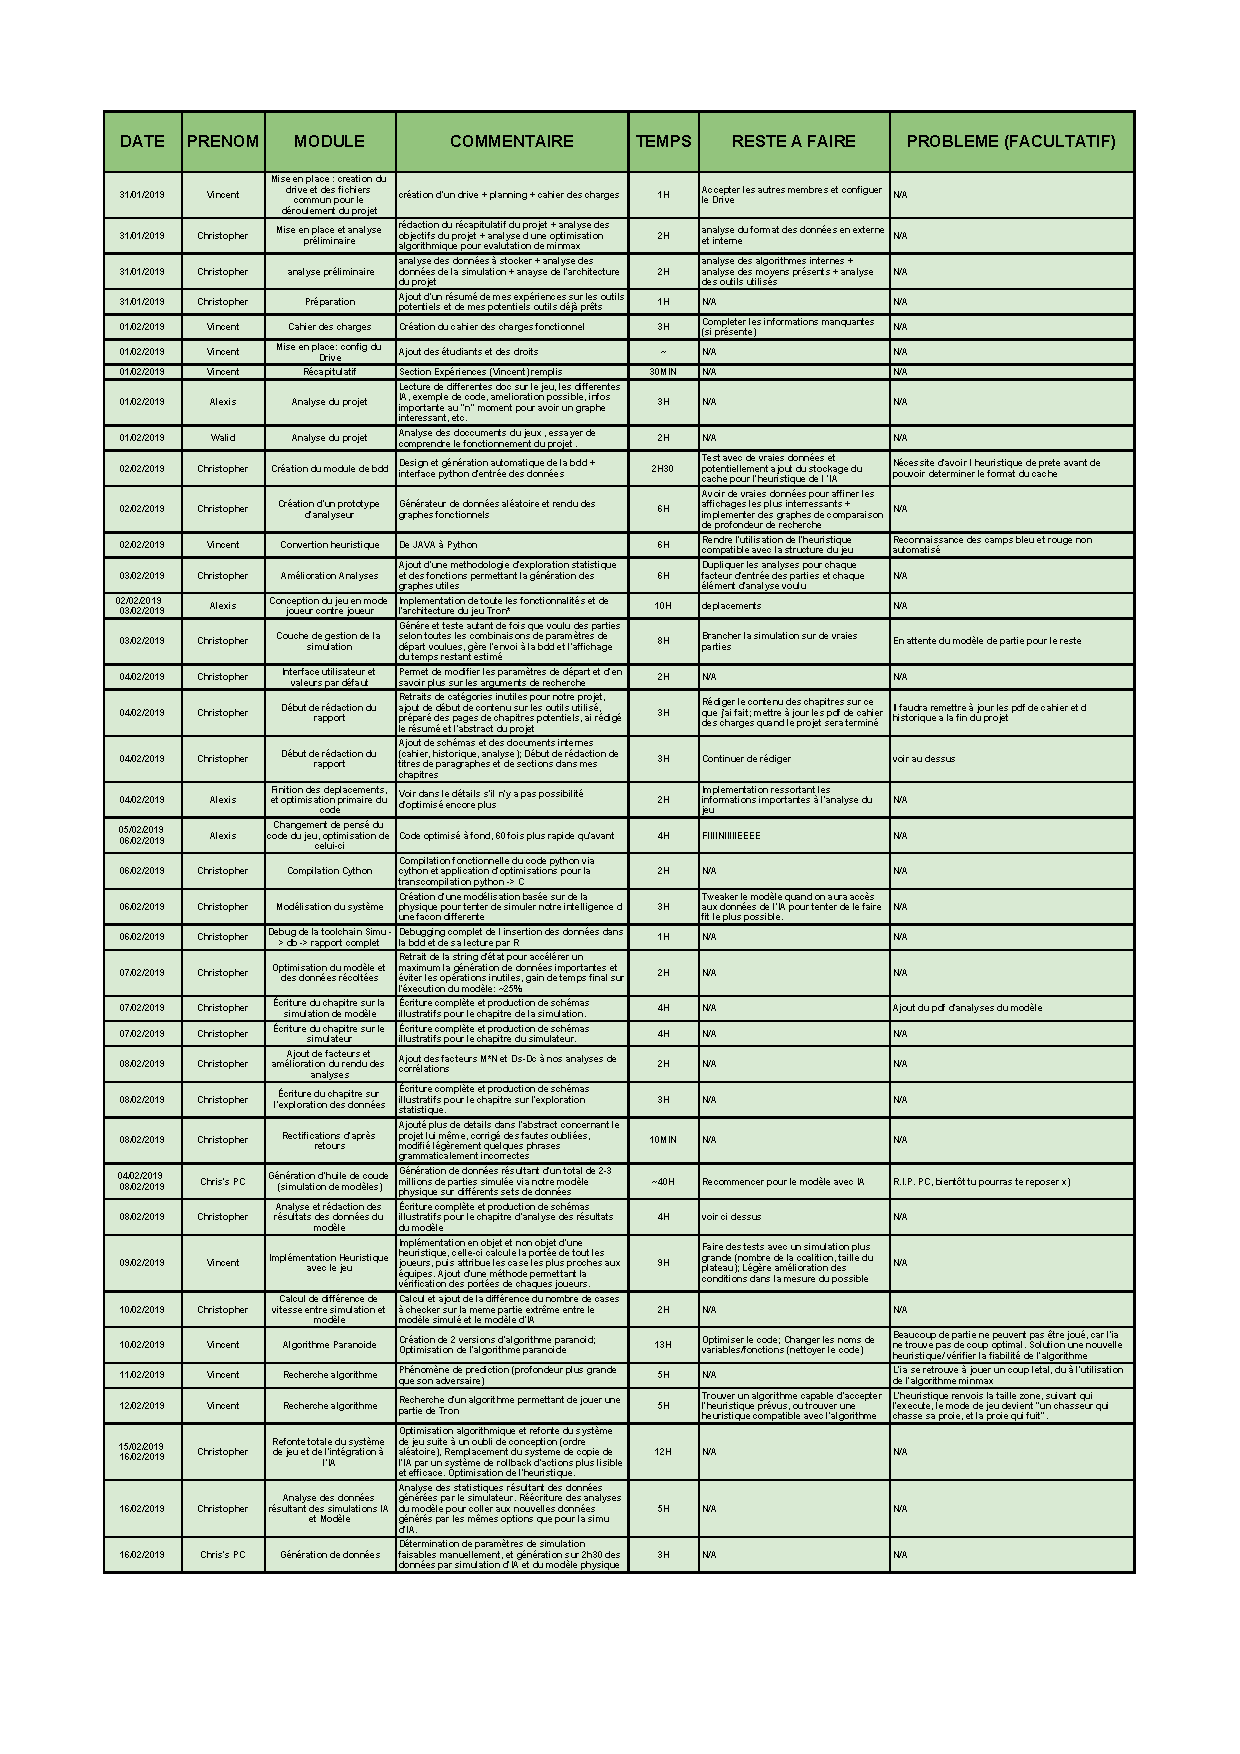
\includepdf[pages=-]{./data/historique.pdf}
		% etc...
		\paragraph{Concernant Walid}
		
		Suite à une discussion sur les expériences, et compétences de chacuns pour analyser comment mener au mieux ce projet, un accord a été passé avec Walid pour qu'il puisse se familiariser de son côté avec Python et aux concepts du projets en tentant d'en réaliser un maximum de son coté.
		
		Afin de ne pas le délaisser non plus, il a été encouragé à poser ses éventuelles questions et à s'inspirer du code principal pour expérimenter et rattrapper son éventuel retard sur certains concepts.
		
		
			\section{Outils de programmation}
				\paragraph{Alexis :}
				\begin{itemize}
					\item IDLE pour coder en python
				\end{itemize}
				\paragraph{Vincent :}
				\begin{itemize}
					\item Vim pour coder en python
				\end{itemize}
				\paragraph{Christopher :}
				\begin{itemize}
					\item Pycharm + l'extension Sonar Lint pour programmer en Python
					\item Rstudio pour programmer le projet en R et étudier le contenu de la base de données
				\end{itemize}
				\paragraph{Walid :}
			
			\section{Bibliothèques utilisées}
				\subsection{Module IA}
				
				\begin{itemize}
					\item random pour jouer des coups aléatoire lors de situations spécifiques.
				\end{itemize}
			
				\subsection{Module simulation}
				
				\begin{itemize}
					\item cython pour compiler et accélerer le temps d'éxécution
					\item PyCallGraph pour une représentation graphique du graphe d'appels, permettant de mieux localiser les endroits à optimiser dans notre programme.
					\item time pour estimer le temps restant avant completion des simulations
					\item sqlite3 pour l'interfacage avec la bdd sqlite
				\end{itemize}
			
				\subsection{Module analyse}
				
				\begin{itemize}
					\item dplyr pour faciliter la manipulation et la selection par sémantique des données
					\item ggplot2 pour ses graphes de qualité et facile à configurer
					\item GGally pour ses outils d'analyse de tables de données complètes
					\item RSQLite pour l'interfacage avec la bdd sqlite
				\end{itemize}
			
		
			
	\part{Réalisation}
	\chapter{Simulateur}

	\section{Nécessités}
	
		\paragraph{Tester de façon uniforme notre espace de recherche}
		Afin de pouvoir avoir des statistiques les moins biaisées possible, il est nécessaire d'uniformiser nos simulations sur notre espace de recherche afin d'éviter la sous-représentation de certains couples de paramètres initiaux.
 
 		
		
	\section{Problème}
		\img{./pics/anal_error.png}
		\paragraph{Comment maximiser la précision statistique d'un couple de paramètre unique?}
		Pour déterminer le poucentage de victoires d'un certain couple de paramètres initiaux, nous allons avoir besoin de réaliser un certain nombre de simulations. 
		
		
		Cependant, quelques tentatives ne serait potentiellement pas représentatif du pourcentage de victoire, un peu comme 3 lancers de pièces ne font pas 50-50 \% de chances d'avoir pile ou face.
		Il nous faudrais donc répeter notre simulation un maximum de fois pour déterminer l'incertitude statistique de notre mesure. Mais combien de fois?
		\img{./pics/anal_margin.png}
		\paragraph{Comment éviter des erreurs d'estimations statistiques?}
		Avec des données mal réparties, nous pourrions avoir des soucis d'estimations. 
		Le graphe représente ci-dessus un exemple de mauvaise représentation potentielle, dûe à la différence de marge d'erreur.
		
		Des données avec les memes marges d'erreurs auraient pu potentiellement au moins retrouver le premier creux en essayant de coller un maximum les points.
		Dans le cas illustré, le calcul pourrais avoir considéré le point haut en incertitude du creux comme une anomalie comparés aux autres points relativement alignés, résultant en une estimation faussée de la forme de nos données.
		
		Évidemment plus de données est toujours mieux pour réduire la marge d'erreur générale de notre estimation, mais comment éviter au moins un maximum cette déformation?
	
		\begin{problem}
			Comment pourrions nous maximiser la précision de nos analyses et la lisibilité de nos résultats?
		\end{problem}
	
	\section{Approches possibles}
	
		\paragraph{Génération aléatoire et uniforme de paramètres initaux}
		Nous pourrions tirer parti de l'aléatoire pour générer de façon aléatoire mais uniformément des couples de paramètres initiaux.
		
		Cela aurait le mérite de pouvoir avoir une image globalement représentative de notre phénomêne avec de moins en moins de déformations dûes à l'aléatoire à mesure que nous multiplions le nombre de tirage au sort de paramètres.
		
		
		Le souci avec cette approche est que nous pourrions potentiellement subir les aléas d'un générateur pseudo aléatoire pas réellement uniforme qui pourrait biaiser nos résultats, et que selon notre espace de recherches, il serait necessaire d'avoir beaucoup de tirages au sorts pour s'assurer de la précision sur certaines données.
		
		
		\paragraph{Génération complète des points de l'espace de recherche}
		L'approche inverse serait de générer exactement toutes les combinaisons possibles de paramètres initiaux de notre espace de recherche, et de les répeter un nombre suffisant de fois pour satisfaire le niveau de précision voulu sur chacun de ces points.
		
		
		La précision de cette approche serait alors directement liée au nombre d'iterations par combinaisons mais aussi potentiellement plus gourmande en simulations que l'approche aléatoire.
	
	\section{Approche utilisée}
	
		\paragraph{Exploration complète d'un espace de recherche voulu}
		
		\begin{result}
			Nous avons préféré partir sur un simulateur parcourant l'intégralité de notre espace de recherche pour minimiser les biais et aléas d'un générateur aléatoire et ainsi maximiser la précision de nos résultats.
		\end{result}
		
		La grande quantité de simulations combinée à la vitesse de calcul du déroulement d'une partie peuvent vite faire durer le processus de génération de données sur plusieurs minutes à plusieurs heures selon l'espace de recherche, mais les données en résultant sont les plus fidèles que nous pourrions avoir en un minimum de temps de génération. 
	
		
	\section{Remarques sur les résultats obtenus}
	
		\img{./pics/simu_speed.png}
		\paragraph{Les performances du modèle de simulation sont critiques}
		La grande quantité de simulations nécessaire pour évaluer un espace de recherche à 5 dimensions sur de petits intervalles à une précision convenable rendent le temps d'execution des simulations cruciales pour générer nos données en un temps raisonnable.
		
		\img{./pics/simu_duration_python.png}
		
		Notre langage de départ étant python, nous avons optimisé notre vitesse d'exécution à l'aide du trancompilateur Cython qui permet de génerer du code C à partir de code source python.
		
		Pour accélerer encore plus nous avons tiré parti de la capacité de Python à intégrer du typage statique via les annotations pour indiquer à Cython les types des variables et le laisser optimiser encore plus profondément les algorithmes C utilisés, en plus d'avoir des indications plus complètes et lisibles pour la documentation en bonus.
		
		
		\img{./pics/simu_duration_cython.png}
		
		\paragraph{Les données sont bel et bien réparties de façon uniforme}
		Grâce à cette approche, nous pouvons bel et bien voir l'uniformité de nos tests sur les paramètres initiaux, la taille maximale de la coalition étant considérée variable selon la taille du plateau, il est cependant normal de voir une densité plus forte de tests plus M et N grandissent, conformément à la taille supérieure de l'intervalles de valeurs C à tester sur ces dimensions d'arène.
		
		Mais même cette augmentation de densité est uniforme.
		Nous pouvons retrouver ce genre d'informations sur les graphes de densités de nos analyses.
		

	\section{Pistes d'amélioration}
	
		\paragraph{Simulations en parallèle}
		Nous avons tenté de faire simuler de multiples simulations en parallèle pour pouvoir profiter des multiples coeurs de nos sytèmes de calculs, mais notre Cython as malheureusement souffert de l'overhead python de la librairie multiprocessing et l'éxecution s'est révélée plus lente que sans.
		
		Une implémentation du multiprocessing directement en C ou via une libraire pyhton déjà optimisée pour Cython devrait permettre d'accélérer grandement les calculs de simulation en parallèlisant la charge de calcul sur autant de coeurs que possibles.
	\chapter{Modèle de jeu}

\begin{info}
	Ce chapitre est actuellement en cours d'écriture.
\end{info}

	%\section{Nécessités}
	
%		\paragraph{but général de l'element}
%		Genre ouais on as besoin d'un moyen de calculer efficacement et rapidement des données de simulation de bonbon qui se font manger pour le projet.
% 
%	
%	\section{Problème}
%	
%		\paragraph{probleme 1}
%		blabla bla vitesse. besoin rapidité mais consomme truc genre memoire.
%		
%		\paragraph{probleme 2}
%		blabla besoin d economiser de la memoire ou un truc mais contraintes de vitesse sinon.
%	
%		\begin{problem}
%			PROBLEMATIQUE QUI COMBINE ET RESUME LES PROBLEMES SUR COMMENT BIEN ALLIER LES DEUX DANS NOTRE CAS.
%		\end{problem}
%	
%	\section{Approches possibles}
%	
%		\paragraph{Approche 1}
%		résumé de ce que c'est, pour et contre, difference avec les autres solutions
%		
%		
%		\paragraph{Approche 1}
%		résumé de ce que c'est, pour et contre, difference avec les autres solutions
%	
%	\section{Approche utilisée}
%	
%		\paragraph{Approche finalement choisie}
%		Les avantages qui ont fait prendre cette décision résumés et plus de details sur les bons cotés de cette décision
%	
%		\begin{result}
%			RESUME DE LA DECISION PRISE
%		\end{result}
%		
%	\section{Remarques sur les résultats obtenus}
%	
%		\paragraph{probleme X}
%		C'etait pas tip top au final comme solution, on as eu un probleme avec X, ce n'etait pas le meilleur des choix et avons rencontré des difficultés que l'on explique rapidement ici.
%		
%	\section{Pistes d'amélioration}
%	
%		\paragraph{meilleures approches}
%		
%		\paragraph{potentielle optimisation}
%		
%		\paragraph{potentiel polissage}
	\chapter{Intelligence Artificielle - Heuristique}

\begin{info}
	Ce chapitre est actuellement en cours d'écriture.
\end{info}

%	\section{Nécessités}
%	
%		\paragraph{but général de l'element}
%		Genre ouais on as besoin d'un moyen de calculer efficacement et rapidement des données de simulation de bonbon qui se font manger pour le projet.
% 
%	
%	\section{Problème}
%	
%		\paragraph{probleme 1}
%		blabla bla vitesse. besoin rapidité mais consomme truc genre memoire.
%		
%		\paragraph{probleme 2}
%		blabla besoin d economiser de la memoire ou un truc mais contraintes de vitesse sinon.
%	
%		\begin{problem}
%			PROBLEMATIQUE QUI COMBINE ET RESUME LES PROBLEMES SUR COMMENT BIEN ALLIER LES DEUX DANS NOTRE CAS.
%		\end{problem}
%	
%	\section{Approches possibles}
%	
%		\paragraph{Approche 1}
%		résumé de ce que c'est, pour et contre, difference avec les autres solutions
%		
%		
%		\paragraph{Approche 1}
%		résumé de ce que c'est, pour et contre, difference avec les autres solutions
%	
%	\section{Approche utilisée}
%	
%		\paragraph{Approche finalement choisie}
%		Les avantages qui ont fait prendre cette décision résumés et plus de details sur les bons cotés de cette décision
%	
%		\begin{result}
%			RESUME DE LA DECISION PRISE
%		\end{result}
%		
%	\section{Remarques sur les résultats obtenus}
%	
%		\paragraph{probleme X}
%		C'etait pas tip top au final comme solution, on as eu un probleme avec X, ce n'etait pas le meilleur des choix et avons rencontré des difficultés que l'on explique rapidement ici.
%		
%	\section{Pistes d'amélioration}
%	
%		\paragraph{meilleures approches}
%		
%		\paragraph{potentielle optimisation}
%		
%		\paragraph{potentiel polissage}
%		
%\chapter{Intelligence Artificielle - Optimisations}
%	
%	\section{Nécessités}
%	
%		\paragraph{but général de l'element}
%		Genre ouais on as besoin d'un moyen de calculer efficacement et rapidement des données de simulation de bonbon qui se font manger pour le projet.
%		
%	
%	\section{Problème}
%	
%		\paragraph{probleme 1}
%		blabla bla vitesse. besoin rapidité mais consomme truc genre memoire.
%		
%		\paragraph{probleme 2}
%		blabla besoin d economiser de la memoire ou un truc mais contraintes de vitesse sinon.
%		
%		\begin{problem}
%			PROBLEMATIQUE QUI COMBINE ET RESUME LES PROBLEMES SUR COMMENT BIEN ALLIER LES DEUX DANS NOTRE CAS.
%		\end{problem}
%	
%	\section{Approches possibles}
%	
%		\paragraph{Approche 1}
%		résumé de ce que c'est, pour et contre, difference avec les autres solutions
%		
%		
%		\paragraph{Approche 1}
%		résumé de ce que c'est, pour et contre, difference avec les autres solutions
%	
%	\section{Approche utilisée}
%		
%		\paragraph{Approche finalement choisie}
%		Les avantages qui ont fait prendre cette décision résumés et plus de details sur les bons cotés de cette décision
%		
%		\begin{result}
%			RESUME DE LA DECISION PRISE
%		\end{result}
%	
%	\section{Remarques sur les résultats obtenus}
%		
%		\paragraph{probleme X}
%		C'etait pas tip top au final comme solution, on as eu un probleme avec X, ce n'etait pas le meilleur des choix et avons rencontré des difficultés que l'on explique rapidement ici.
%		
%	\section{Pistes d'amélioration}
%	
%		\paragraph{meilleures approches}
%		
%		\paragraph{potentielle optimisation}
%		
%		\paragraph{potentiel polissage}
	\chapter{Analyse - Exploration}

	\section{Nécessités}
	
		\paragraph{Déterminer les facteurs d'une victoire}
		L'objectif final de ce projet est de déterminer les meilleurs paramètres initiaux permettant de maximiser le taux de victoires de la coalition.
		
		Cela étant dit, notre objectif pour y parvenir est d'utiliser l'outil de l'analyse statistique, mais sur les données d'un demi-million de parties potentielles avec une demi douzaine de facteurs différents, par où commencer?
 
	
	\section{Problème}
		
		\paragraph{Comment déterminer les bonnes corrélations?}
		Faire des statistiques à partir de l'intégralité de nos données permet de déterminer des tendances générales, mais sur notre cas où nous avons 5 dimensions de données indépendantes, et donc potentiellement des variations de ces corrélations à chaque modification infime de n'importe quel facteur, comment pourrions nous analyser relativement efficacement l'évolution de ces tendances pour tenter de déterminer de potentielles corrélations cachées entre plusieurs variables?
		
		\img{./pics/anal_partial.png}
	
		\begin{problem}
			Comment pourrions-nous analyser nos données pour pouvoir y déceler des informations de la façon la plus efficace et complète possible sur autant d'axes?
		\end{problem}
	
	\section{Approche utilisée}
	
		\paragraph{Analyse par tranches}
		La quantité inconnue de données que nous avons pour chaque variable, construire une matrice à 5 dimensions serait prohibitif pour nos moyens actuels, autant en espace mémoire qu'en temps de calcul, d'analyse et de génération.
		C'est pour cette raison que nous avons opté pour une simple analyse par intervalles de données présentes.
	
		\begin{result}
			Analyser les tendances de victoire en fixant une variable ou plusieurs variables à la fois et en scindant nos données en 5 intervalles de tailles équivalentes nous permet d'analyser la progression des spectres entre de grandes variations des variables en questions et d'avoir une idée générale des relations entre variables.
		\end{result}
	
		\img{./pics/anal_tranches}
		
	\section{Remarques sur les résultats obtenus}
	
		\paragraph{Les données sont parlantes}
		Voir progresser les intervalles de données disponibles en fonction des intervalles de chaque variable et les voir se chevaucher petit à petit permet vraiment d'avoir une meilleure idée de ce que représente chaque intervalle dans la totalité des données présentes.
		De plus, la comparaison aisée entre les différents spectres à différents intervalles montrent bel et bien si les spectres changent beaucoup ou non selon tel ou tel intervalle d'une variable et permet de déterminer l'influence de cette variable sur ces spectres ou non.
		
	\section{Pistes d'amélioration}
	
		\paragraph{Génération d'un profil 5D voire n-D de probabilités!}
		Comme dit plus haut, à partir de ce genre de données il paraitraît tout naturel de tenter de modéliser un spectre 5D de probabilités permettant de déterminer automatiquement la probabilité de victoire d'un couple de paramètres initiaux arbitraires.
		
		Cela pourrait d'ailleurs être un sujet bien chargé très intéressant à implémenter et à travailler qui pourrait permettre de s'intéresser à des sujets peu communs comme les tenseurs et l'interpolation!
		

		
	\part{Analyse des données générées}
	
	\chapter{Analyse des données de l'IA}

\paragraph{Paramètres initiaux}
Cette simulation as été réalisée avec 100 réitérations pour chaque combinaison possible avec les paramètres suivants.
\img{./data/ai_parameters}

\begin{info}
	On remarquera que la profondeur de recherche as une petite fourchette dans notre espace de recherche pour des raisons de temps de calcul. Une analyse plus poussée dans de petites cartes pourrait être intéressante.
\end{info}

\section{Analyse d'ensemble}
\img{./data/ai_overview_short}
\paragraph{Des données très localisées}
Nous pouvons d'abord remarquer la présence de trois groupes de données bien distincts:
\begin{itemize}
	\item Un groupe de paramètres à la victoire quasiment garantie
	\item Un groupe de paramètres à la défaite quasiment garantie
	\item Un groupe de paramètres plus étalé mais avec de faibles chances de victoire
\end{itemize}

Les facteurs M,N, C et area semble n'avoir aucune influence sur le pourcentage de victoire.

En revanche, il est intéressant de noter que Dc, Ds, et leur différence semblent fortement influer sur ce pourcentage.


\img{./data/ai_overview_complete}

\section{Analyses détaillées}
\subsection{Répartitions des pourcentages de victoires}
\img{./data/ai_victory_percent}
\paragraph{La différence d'intelligence semble être primordiale}
Les victoires semble être principalement réparties sur des couples de paramètres où la coalition et le joueur solo sont aussi intelligents, ainsi que lorsque Ds et Dc sont plus élevés.

La répartition en M, N, C et area est homogène parmi les pourcentages de victoire, donc ne semblent pas influer sur le résultat d'une partie.


\subsection{Découpage du spectre selon des intervalles de C}
\img{./data/ai_C}
\paragraph{Aucune variation particulière}
Malgré le manque de données empêchant la détermination de courbes, l'aspect général des spectres ne varie pas selon C.


\subsection{Découpage du spectre selon des intervalles de Dc}
\img{./data/ai_Dc}
\paragraph{Une scission importante}
Dc influe clairement sur les pourcentages de victoire, sur notre set de données, une haute valeur de Dc semble garantir la victoire. 


\subsection{Découpage du spectre selon des intervalles de Ds}
\img{./data/ai_Ds}
\paragraph{Une autre scission importante}
Ds semble influer aussi beaucoup sur le résultat d'une partie, une faible valeur de Ds semble garantir la défaite de la coalition, tandis que des valeurs plus grandes semblent faire émerger des groupes selon la différence d'intelligence.


\subsection{Découpage du spectre selon des intervalles de l'aire M*N}
\img{./data/ai_area}
\paragraph{Aucune variation particulière}
Nous ne pouvons pas constater de variation particulière des spectres en fonction de l'aire du plateau. Celui ci ne semble donc pas influer sur les chances de victoire.

\subsection{Découpage du spectre selon des intervalles de la différence de niveau}
\img{./data/ai_Dc-Ds}
\paragraph{Des groupes intéressants}
À faible différence d'intelligence, nous pouvons voir que M,N,C et area semblent parfaitement équilibrés, et la différence soudaine de chances de victoires entre de faibles valeurs de Ds, Dc, et de plus grandes valeurs de Ds, Dc.

En revanche à plus grande différence d'intelligence, les chances de victoires semblent être plus constantes et plutôt faibles, sur toutes les combinaisons de valeurs. 

\subsection{Conclusions d'analyse}

\paragraph{À niveau égal, rien ne va plus!}
D'après nos résultats, nous pouvons constater que plus la différence relative d'intelligence est petite, plus la coalition as de chances d'écraser le joueur solo, et ce indépendamment du nombre de joueurs ou de la taille de la carte.

Cependant, notre fourchette de donnée est limitée concernant les différentes valeurs d'intelligence, et une analyse plus poussée sur ces variables là en particulier, suite à des optimisations nécessaires, pourrait permettre d'y voir plus clair. 

\begin{result}
	 À intelligence proche, la coalition semble invincible.
\end{result}

\img{./data/ai_conclu}
	\chapter{Analyse des données du modèle}

\paragraph{Paramètres initiaux}
Cette simulation as été réalisée avec 100 réitérations pour chaque combinaison possible avec les paramètres suivants.

\img{./data/model_parameters}

\section{Analyse d'ensemble}


\img{./data/model_overview_short}
\paragraph{Quelques facteurs sortent du lot}
À commencer par le facteur C qui est le seul avec une fonction qui tends vers 1 si rapidement, les mesures d'espace M, N et M*N semblent avoir aussi une corrélation positive avec le pourcentage de victoire.

La tendance de Dc à réduire le pourcentage de victoire avant un certain point est aussi étonnante, on pourrais penser que plus de prévoyance de la part des joueurs en groupe puissent les avantager, mais on dirais qu'il y a un certain équilibre entre prévoyance et hasard qu'il leur faut conserver pour être efficace. 
On retrouve la même tendance étonnante sur la courbe de différence d'intelligence, où réduire la différence au minimum comme de la maximiser semble porter les meme résultats.


Le facteur ds semble coller à nos attentes en revanche, plus le joueur solo est intelligent, plus les chances de gagner semblent diminuer en général, même si l'incertitude actuelle ne nous permets pas d'être certains de cette tendance.


\img{./data/model_overview_complete}

\section{Analyses détaillées}
\subsection{Répartitions des pourcentages de victoires}
\img{./data/model_victory_percent}

\paragraph{Une évolution qui suit la distribution de C}
Les axes en Y étant fixes entre les différents intervalles de victoires, nous pouvons bel et bien constater sans déformation plusieurs ensembles de données.

Les parties à 60-\% de chances de victoire ont une répartition relativement homogème sur les differents spectres excepté sur le facteur C, qui indique très clairement que toutes les valeurs de petit C sont en deçà de 60\% de chances de victoire.
De même pour les variables M, N et area, le centre de leur distribution dépends du pourcentage de victoire, plus il y as d'espace, plus il y a de victoires.

Les distributions homogènes des autres spectres selon les différents pourcentage de victoire montrent que ceux ci ne semblent pas influencer l'issue des parties.



\subsection{Découpage du spectre selon des intervalles de C}
\img{./data/model_C}
\paragraph{C est définitivement un facteur MAJEUR}
Cette représentation montre bien l'écrasante influence de C sur le pourcentage de victoire, aussitôt une valeur (minime en plus) atteinte, les chances de victoires enregistrées sont quasiment assurées.
Autrement, nous retrouvons les fonctions du départ mais plus proche de la neutralité qu'au-dessus.
Voire parfois les fonctions semblent stagner à ces faibles valeurs de C.




\subsection{Découpage du spectre selon des intervalles de Dc}
\img{./data/model_Dc}
\paragraph{Aucun impact réel décelé}
Dc ne semble vraiment pas influer sur les différents spectres, par conséquent, Dc ne semble pas avoir d'impact tout court sur notre distribution de probabilité.



\subsection{Découpage du spectre selon des intervalles de Ds}
\img{./data/model_Ds}
\paragraph{Aucun impact réel décelé non plus}
Ds ne semble vraiment pas influer sur les différents spectres non plus, par conséquent, Ds ne semble pas avoir d'impact tout court sur notre distribution de probabilité.


\subsection{Découpage du spectre selon des intervalles de l'aire M*N}
\img{./data/model_area}
\paragraph{Une tendance positive!}
Plus la zone d'aire augmente, plus on peut voir les points et les fonctions se décaler vers la victoire.
Sur M on peut même voir petit à petit les points les plus bas disparaitre au fur et à mesure. 

\begin{info}
	Cela peut s'expliquer par la correlation suivante: Plus l'aire est grande, plus la taille de la coalition peut l'être aussi, résultant naturellement vers de meilleures chances de victoire. Car plus de joueurs implique aussi plus de contrôle global du plateau.
\end{info}



\subsection{Découpage du spectre selon des intervalles de la différence de niveau}
\img{./data/model_Dc-Ds}
\paragraph{Toujours aucun impact réel décelé}
La différence d'intelligence ne semble pas non plus influer particulièrement sur les chances de victoires.


\subsection{Conclusions d'analyse}
\paragraph{Le contrôle de la carte est le facteur le plus important d'après notre modèle}
La seule véritable corrélation que nous ayons pu déceler ici entre variables et pourcentages de victoire est en fonction du nombre de joueurs présents sur la carte.

Si nous y réfléchissons bien, cela fait même sens! 

\begin{result}
	Avec une stratégie purement défensive, et un unique joueur dans son équipe, un joueur seul as plus de chance d'éliminer son équipe sur la durée qu'une équipe nombreuse jouant aussi en pure défensive et contrôlant plus de surface au total.
\end{result}

\img{./data/model_conclu}
	%\includepdf[pages=-]{./data/analyse}
	
	\part{Problèmes, tests et expérimentations}
	
				
			
		\chapter{Conclusion}
		
		\begin{info}
			Nous n'avons pas reçu de réponses de la part de Walid pour ses conclusions.
		\end{info}
		
		
		
			\section{Résumé des objectifs au résultat final}
			
			
			\begin{problem}
				Le but est d'analyser les meilleurs paramètres pour que notre coalition soit statistiquement la plus efficace contre le joueur seul, si une tendance se dégage de nos simulations.
			\end{problem}
			
			
			\paragraph{Citons les résultats finaux de nos analyses:}
			
			D'après nos analyses finales sur un échantillon de 12000 simulations, nous avons pu déterminer que:
			
			\begin{itemize}
				\item La pire coalition possible serait une coalition qui joue quasiment au hasard, avec peu d'équipiers et sur une grande carte.
				\item La coalition idéale semble être une coalition en surnombre, d'intelligence égale au joueur solo, et sur une petite carte.
			\end{itemize} 
			
			De plus, sur toute carte moyenne ou petite, la coalition est statistiquement meilleure. 
			
			
									
			\section{Enrichissement personnel}
				\subsection{Vincent: }
				\paragraph{}
				Ce projet m'as permis de découvrir plusieurs phénomène sur l'algorithme MinMax. 
				J'ai beaucoup appris sur l'impacte que peut avoir une heuristique sur un algorithme. 
				J'ai pu me documenter sur plusieurs autres algorithmes. Réaliser tout ces optimisations pour le modules d'analyse, m'a fait comprendre que l'on peut passer par d'autre chemin pour un résultat identique mais plus rapide.
				Travailler avec ce groupe m'as permis d'apprendre de nouvelle méthode de travail, et aussi des nouveaux outils en informatique.
				 
				\subsection{Alexis:} 
				\paragraph{}
				Ce projet à été enrichissant sur le plan informatique comme sur le plan humain. En effet, j'ai pu découvrir des méthodes de travail différentes des miennes et ai améliorer ma capacité à  travailler en groupe. 
				Nous avons bien su nous entendre et sommes arrivé à un résultat plus que satisfaisant. 
				
				Sur le plan informatique j'ai pu approfondir mes connaissances et mes réflexions en optimisation, comment rendre/adapter le code au besoin en faisant des choix et des compromis pour trouver le juste milieu entre rapidité efficacité et flexibilité. 
				
				J'ai aussi découvert les limites et les contraintes des IA, surtout sur minmax où l'effet d'horizon m'était inconnue et où le choix de notre heuristique était importante pour permettre aux analyses d'être efficace.
				 
				\subsection{Christopher:} 
				\paragraph{}
				Ce projet m'as beaucoup appris, en très peu de temps j'ai pu me familiariser avec les particularités de cython, et expérimenter avec.
				Les nombreuses fouilles à l'optimisation ont été un bonheur de problèmes à creuser et les accélérations progressives encourageaient à toujours creuser plus loin.
				
				De même, m'étant familiarisé avec R aux alentours de Décembre 2018 pour des projets extra-scolaires, le travail sur la représentation finale des données fut long et riche en apprentissages.
				De nombreux volontaires ont participé aux critiques sur les différentes itérations de celles ci pour améliorer la compréhensibilité ainsi que la clarté en recherchant jusqu'aux couleurs visibles pour des daltoniens, à la recherche des données les plus pertinentes et intuitives sur l'intégralité de nos données, et un travail de représentation de celles ci pour en rendre la lecture la plus naturelle possible. 
				
				Nous espérons que la représentation finale y fasse honneur.
	 
						
			\section{Perspectives envisagées, appréciation perso, poursuite..}

				 
				\subsection{Vincent: } 
				\paragraph{}
				Nous pourrions utiliser l'algorithme Monte-Carlo pour gagner du temps de calcul. 
				Ce qui permettrait de supprimer l'heuristique, qui possède une très grande importance dans l'algorithme. 
				Imaginer une solution sans heuristique permettrait d'enlever plusieurs problème.
				
				Mener une étude sur les positions idéal que pourrait avoir les joueurs sur le plateau serait très enrichissant.

				\subsection{Alexis:} 
				\paragraph{}
				
				Afin d'ameliorer notre code, je pense qu'il pourrait etre judicieux de le refaire en C afin de pouvoir optimiser la rapidité de celui-ci en adapatant vraiment le code a la machine utilisé pour que celle-ci puisse faire des analyses  de masse beaucoup plus rapide.  Pour l'IA nous avons beaucoup parlé de l'algorithme Monte-Carlo qui nous ferait gagner beaucoup de temps de calcul.
				
				J'ai beaucoup aimé travaillé avec ce trinome, Vincent et Christopher sont malin, intéressé, motivé et très intelligent, je crois bien que c'est le premier groupe avec lequel j'ai pris plaisir à travailler

				\subsection{Christopher:} 
				En travaillant sur ce projet, notre groupe s'est souvent repenché sur le sujet de l'approche de Monte Carlo. 
				La voyant repasser depuis quelques années déjà au cours des recherches sur divers projets, et ayant étudié les explications sur le concept via sa page wikipédia anglophone, j'aimerais beaucoup tenter de l'appliquer lors d'un projet futur pour expérimenter avec et vraiment être certain de saisir le concept.
				
				Les optimisations semblent aussi être un domaine fascinant, et je creuserais très certainement le concept dans le futur.
				
				Sur un autre sujet, cette équipe est probablement la meilleure équipe avec laquelle j'aie pu travailler: motivée et intéressée. 
				J'espère sincèrement pouvoir retrouver tout le monde en master l'année prochaine et avoir l'occasion de refaire des projets de ce style plus souvent!
				


			\cleardoublepage
			\pagebreak
		\pagenumbering{Roman}
			
		\part{Annexes}
		
		\chapter{Analyse - Simulation}
	
	
	\section{Nécessités}
	
		\paragraph{Tenter de modéliser un système à priori intelligent}
		Les calculs d'heuristique sont chers, et il est parfois utile pour optimiser la prédiction ou la detection d'anomalies de tenter de trouver un modèle mathématique qui décris bien l'évolution de notre système.
		
		Mais si les calculs d'heuristiques sont chers, ils sont malheureusement au premiers abord nécessaires, pour pouvoir observer des phénomènes dans leur globalité avant de tout analyser. Pour tenter de trouver un modèle il va donc falloir beaucoup de données pour trouver de potentielles corrélations reccurentes.
 
	
	\section{Problème}
	
		\paragraph{À quel point telles données sont elles pertinentes?}
		Afin de pouvoir affiner notre modèle et le faire ressembler un maximum au comportement de notre véritable phénomène, il est important de déterminer l'importance de chaque facteur dans son comportement.
		
		Comment déterminer par la suite l'équivalence de cette importance dans notre autre visualisation du problème? Sont-elles comparables?
		
		\paragraph{Quels types de modèles pouvont nous créer?}
		Il existe une infinité de fonctions possibles, correspondant à notre profil recherché sur notre intervalle de données.
		Si notre modèle doit être capable d'extrapoler, l'intuition et les analogies au monde physique peuvent-ils être suffisants? 
		
		La réponse à cette question est évidemment complexe. Mais aussi évidente: On ne peut pas prédire avec exactitude quelque chose sur laquelle nous n'avons aucune donnée. 
		Par conséquent, il va falloir partir du principe que les données suivantes ressembleront à une tendance connue qui corresponds déjà aux données présentes.
		
		Mais comment déterminer laquelle?
	
		\begin{problem}
			Comment pourrions-nous déterminer un type de modèle et ses paramètres pour représenter le même comportement que notre phénomène connu ?
		\end{problem}
	
	\section{Approches possibles}
	
		\paragraph{Mathématiques pures}
		Avec des mathématiques pures, et à partir de suffisamment de données d'entrées, nous devrions pouvoir construire un spectre de probabilités de victoire en fonction des paramètres initiaux.
		
		Cela devrait permettre une prédiction des plus fidèles de notre comportement sur l'intervalle connu, mais l'extrapolation sur un spectre de probabilités nous semble être d'un très haut niveau de mathématique que nous n'avons malheureusement pas dans notre équipe.
		
		La prédiction en données connues serait donc instantanée mais l'extrapolation impossible.
		
		\paragraph{Modèle simulé inspiré par la physique}
		Avec de la physique il est possible de tenter de raisonner différemment, et de calculer potentiellement plus rapidement le meme genre de résultats que le calcul complet de notre phénomêne de départ.
		
		De plus, cela permettrais aussi potentiellement de mettre en équation le comportement des acteurs de notre phénomêne, ici les IA, et de potentiellement trouver un modèle simplifié et fonctionnel pour leur heuristique.
		
		Ici les équations pourraient permettre de l'extrapolation relativement aisément, mais la précision de notre modèle va nécessiter un lourd travail de réglages pour trouver l'équilibre entre l'influence des paramètres dans le modèle des IA et celle sur les paramètres dans le modèle simulé. 
		
		Un exemple parlant est la traduction de l'influence de la profondeur de recherche des IA vers le modèle physique, où il n'y aura pas d'IA.
	
	\section{Approche utilisée}
	
		\paragraph{Modèle physique}
		Le temps et l'expérience limitée des membres du groupe dans le domaine de la simulation nous ont forcés à partir pour le modèle inspiré de la physique.
		\img{./pics/simu_prof.png}
		Nous avons donc pris les joueurs pour des billes (littéralement), et les considérons désormais en roulis perpétuel vers la pente la plus accentuée qui s'offre à eux.
		
		À la suite de leur roulis (changement de case), un mur se crée à leur position actuelle, les forcant à continuer de rouler au tour suivant.
		
		\img{./pics/simu_depth.png}
		Ces murs sont de matériau friable, comme du sable, et une fois posés, remplissent les trous environnants d'une légère quantité de sable sans jamais les boucher, réduisant ainsi leur pente.
		
		Une bille ne peut plus rouler si elle est entourée de murs, autrement dit, si elle n'as plus de pente sur laquelle rouler.
		Elle est alors retirée du jeu et considérée hors jeu.
		
		\img{./pics/simu_avoid.png}
		Ce système devrais favoriser le contrôle de la carte de façon naturelle, car les billes seront donc naturellement inclines à se diriger vers les endroits les plus profonds, c.à.d. ceux ayant le plus d espace libre, et continueront toujours de rouler tant qu'elles n'auront pas atteint de cul de sac.
		
		Pour tenter de donner une dimension d'équipe, nous avons attribués une légère force attirant la coalition vers la position du joueur pour départager deux cases de même profondeur.
		
		Un barycentre de force pourrait être nécessaire pour calculer la force inverse pour le joueur seul, et cela nous as semblé potentiellement trop coûteux en temps de calculs supplémentaires pour rendre le modèle potentiellement viable.
		L'idée reste à tester.
		

		\begin{info}
			Ce modèle est basé sur l'heuristique de base du projet, qui est la maximisation de la surface contrôlée par les équipes à chaque tour. L'IA a évolué depuis.
		\end{info}
		
	\section{Remarques sur les résultats obtenus}
	
		\paragraph{Des résultats qui ne collent pas à notre modèle IA}
		Notre physique semble être trop indépendante de l'intelligence des joueurs, les données de l'IA nous montrent un différence plus porté sur l'écart d'intelligence que sur le reste.
		
		Ceci est surement explicable par le fait que ce modèle joue sur un principe purement défensif tandis que notre IA alterne parfois entre défense et aggression.
		\begin{result}
			Il serait peut être possible cependant d'utiliser notre modèle en optimisation pour les IA en totale autarcie et économiser en temps de calcul quand aucune stratégie offensive n'est désormais utile.
		\end{result}
	
		\paragraph{Un semblant de stratégie!}
		Nous avons pu constater que malgré l'absence de prédiction de la part des billes, celles ci semblaient avoir parfois des semblants de stratégies, par exemple, nous avons pu surprendre le joueur solo à coincer un adversaire dans un couloir de deux cases puis lui faire une queue de poisson en sortie!
		
		Même sans prédiction, nous arrivons donc à recalculer des mouvements potentiellement stratégiques, il y a donc espoir de pouvoir affiner notre modèle plus encore.
		
		\paragraph{Une optimisation de temps de calcul efficace!}
		Là où notre IA est forcée de calculer la zone de contrôle d'un joueur jusque $3^C*Ds$ fois dans le pire des cas (tous les joueurs peuvent aller dans 3 directions à chaque tour, sur Ds tours), sur l'intégralité de la carte importante pour chaque joueur simulé à chaque simulation, notre système se contente d'un rayon de recherche de profondeur qui calcule en une fois l'intérêt d'une case et de ses alentours, et ce sur les quatre cases adjacentes à la bille.
		
		Le calcul de la zone ne néglige les cases inutiles et donc s'arrête soit en cas de rayon atteint, soit en cas d'obstacle atteint dans sa propagation de comptage, ce calcul peut donc être de complexité O(1) en cas d'encerclement et sa moyenne baisse à mesure que le nombre de murs augmente.
		
		\img{./pics/simu_efficiency.png}
		À contrario, la recherche pour notre IA nécessite de calculer et propager autant de zones que de joueurs, incluant donc une plus grande surface à propager pour le calcul des zones d'un seul joueur, lors d'une unique étape de simulation.
	
	\section{Ordre de grandeur de la différence de vitesse de calcul}
		\begin{figure}[H]
			\centering
			\begin{tabular}{c c c c c}
				M&N&C&Ds&Dc\\\hline
				50&50&36&10&9\\				
			\end{tabular}
		\caption{Paramètres initiaux}	
		\end{figure}
		
		\paragraph{Des paramètres initiaux extrêmes}
		Cette partie est la partie la plus extrême de notre échantillon de données sortant de notre simulation modélisée, en sachant que celles ci ont toutes été répétées 100 fois pour avoir une certaine précision.
		Nous allons ici tenter d'estimer à grand renfort d'approximations la quantité de cases touchées par nos calculs pour la décision de nos joueurs afin de pouvoir comparer la différence d'efficacité entre nos deux modèles. 
		
		\paragraph{Les constantes}
		Nous déterminons d'abord les constantes qui nous serviront à simplifier nos équations:
		\begin{itemize}
			\item $D$ représente la profondeur moyenne de recherche des joueurs
			\item $t_{max}$ représente le nombre maximum de tours pouvant être joués si personne ne meurt tout le long de la partie.
		\end{itemize}
	
		
		\begin{align}
		D &= \frac{C*Dc+1*Ds}{C+1}\\
		&\approx 9 \\
		t_{max} &= \frac{M*N}{C+1}\\
		& \approx 68
		\end{align}
		
		\subsection{Modèle IA}
		
		
		
		\begin{align}
			nbCases(t, M, N, C) &= M*N-(C+1)*t\\
			nbCases(t) & = 2500 - 37 * t\\
			nbCases/tour/joueur(t, D) &= \int_{t}^{t+D} nbCases(x) dx\\
			&= [2500*t - 37*\frac{t^2}{2}]_{t}^{t+D}\\
			& = 2500(t+D-t) - 37*\frac{(t+D-t)^2}{2}\\
			nbCases/tour/joueur(D)& = 2500*D - \frac{37}{2}*D^2\\
			totalCases(t_{max}, C, D) &= (C+1)*t_{max}*nbCases/tour/joueur(D)\\
			&= (C+1)*t_{max}*(2500*D - \frac{37}{2}*D^2)\\
			&= 37*68 *(2500*9 - \frac{37}{2}*9^2)\\
			&= 2516 * (22500 - 18.5*9^2)\\
			&= 2516 * (22500 - 1498.5)\\
			&= 2516 * 21001.5\\
			totalCases(t_{max}, C, D) &\approx 52839774
		\end{align}
		
		\subsection{Modèle simulé}
		
		\begin{align}
			nbCasesInRadius(D) &=\int_{0}^{D} 4*x dx\\
			&= [4\frac{x^2}{2}]_{0}^{D}\\
			nbCasesInRadius(D) &= 2D^2\\
			totalNbMurs(t,C) &= t*(C+1)\\
			ratioMur/case(t, M, N, C)&= \frac{totalNbMurs}{M*N}\\
			ratioMur/case(t, M, N, C)&= \frac{t*(C+1)}{M*N}\\
			nbMurInRadius(t,M,N,C,D)&=ratioMur/case(t, M, N, C)*nbCasesInRadius(D)\\
			nbMurInRadius(t,M,N,C,D)&=\frac{t*(C+1)}{M*N}*2D^2\\
			casesLibreInRadius(t,M,N,C,D)&=nbCasesInRadius(D) - nbMurInRadius(t,M,N,C,D)\\
			casesLibreInRadius(t,M,N,C,D)&=2D^2-\frac{t*(C+1)}{M*N}*2D^2\\
			casesLibreInRadius(t,M,N,C,D)&=2D^2*(1 - \frac{t*(C+1)}{M*N})\\
			nbCases/player/turn(t,M,N,C,D) &= 3*casesLibreInRadius(t,M,N,C,D)\\
			&= 3*2D^2*(1 - \frac{t*(C+1)}{M*N})\\
			nbCases/player/turn(t,M,N,C,D) &= 6D^2*(1 - \frac{t*(C+1)}{M*N})\\
			nbCases/turn(t,M,N,C,D) &= (C+1)*nbCases/player/turn(t,M,N,C,D)\\
			nbCases/turn(t,M,N,C,D) &= (C+1)*6D^2*(1 - \frac{t*(C+1)}{M*N})\\
			totalCases(t_{max},M,N,C,D) &= \int_{0}^{t_{max}} nbCases/turn(t,M,N,C,D) dt\\
			&= (C+1)*6D^2* \int_{0}^{t_{max}} 1 - \frac{t*(C+1)}{M*N} dt\\
			&= (C+1) * 6D^2 * [ t - \frac{(C+1)}{M*N} * \frac{t^2}{2} ]_{0}^{t_{max}}\\
			&= (C+1) * 6D^2 * (t_{max} - \frac{(C+1)*t_{max}^2}{2*M*N})\\
			&= 37 * 486 *(68 - \frac{37*68^2}{5000})\\
			&= 17982 * (68 - 34)\\
			totalCases(t_{max},M,N,C,D) &= 611388
		\end{align}
		
		\subsection{Comparaison des deux modèles}
		
		\paragraph{Nous pouvons calculer notre speedup}
		Grâce aux résultats ci dessus, nous pouvons calculer le speed up entre nos deux modèles.
		
		\begin{align}
			\frac{totalCases_{IA}}{totalCases_{simu}} &= \frac{52839774}{611388}\\
			\frac{totalCases_{IA}}{totalCases_{simu}} &\approx 86 
		\end{align}
		
		\begin{result}
			Pour ce cas extrême, notre simulation teste 86 fois moins de cases que notre IA de base. C'est énorme.
		\end{result}
	
	\section{Pistes d'amélioration}
	
		\paragraph{Un meilleur réglage des facteurs du modèle}
		Pour le moment nous avons considéré les facteurs de notre modèle relativement linéairement à partir des paramètres initiaux mais l'IA peut potentiellement réagir à d'autres facteurs que nous pourrions peut etre quantifier pour améliorer notre modèle.
		
	
	
\end{document}
